\documentclass[11pt]{article}
%Gummi|061|=)
\title{\textbf{Welcome to active-data}}
\author{Hagen Geissler\\
		Your Name}
\date{}
\usepackage{graphicx}
\begin{document}

\maketitle

\section{Before you start}

Try to mentally step back for a second and imagine you standing infront of a 100 gigabyte data chunk format JSON,\\
rock solid painted in black.\\\\
Your existence depends on finding the little data Nugget who lives in GigaByte 52.17 
you never seen the thing bevor,
what do you do. 



\section{AI-micro-structures}
They are called like that because they have multiple properties some are related to the nugget you still searching. The name giving properties come from the genetic way the data is organised.


\begin{figure}[htp]
\centering
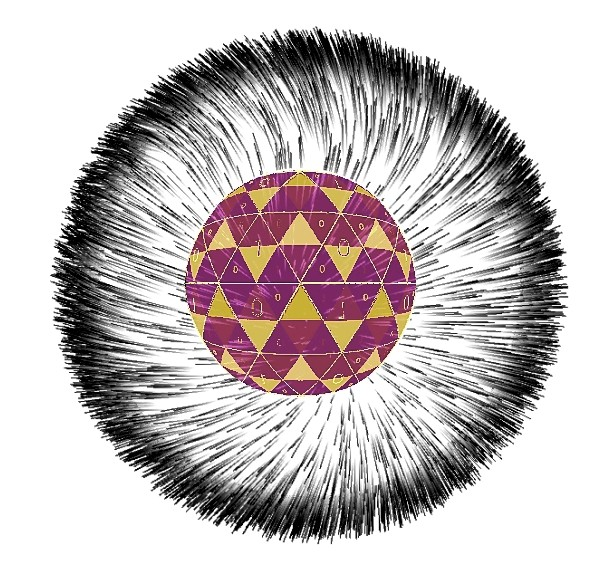
\includegraphics[scale=0.29]{./image/artee-0.jpg}
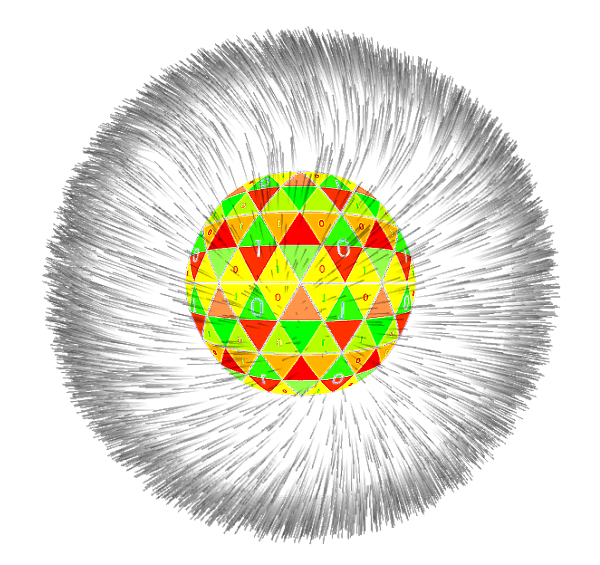
\includegraphics[scale=0.29]{./image/artee-1.png}
\caption{}
\label{}
\end{figure}


\section{Optimized data-surface}
\begin{figure}[htp]
\centering
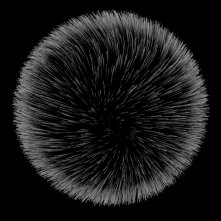
\includegraphics[scale=0.59]{./image/query-surface.jpg}
\end{figure}
\subsection{Data Restructure}

\begin{itemize}
\item Each knot in the data structure is identified
\item same query distance for each knot in the structure
\end{itemize}
\subsection{Fitness}


\begin{itemize}
\item querying based on a matrix within a semantic domain
\item data fitness based on query matrix


\end{itemize}

\subsection{Data States}

\begin{itemize} 
\label{item any mix of states}
\item born \item pampered  \item growing 
\item become adult \item get wise \item die
\item unknown
\item semantically signed
\end{itemize}



\section{Concept's}
\begin{figure}[htp]
\centering
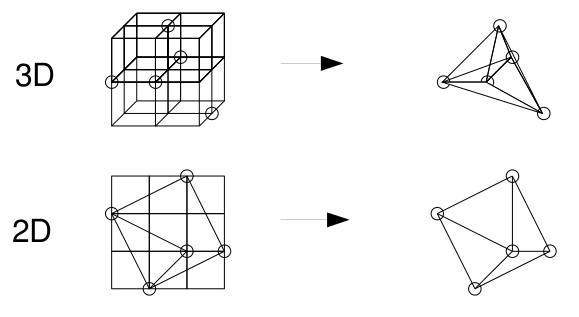
\includegraphics[scale=0.65]{image/research-base-002.png}
\caption{}
\label{}
\end{figure}



\section{Feedback}
contact me at: \emph{http://santex@cpan.org}
\\
join the project:\\
\emph{https://github.com/santex/active-memory} 
\\
\emph{http://coderwall.com/teams/4f901f4462db21000a000005}


\begin{figure}[htp]
\centering
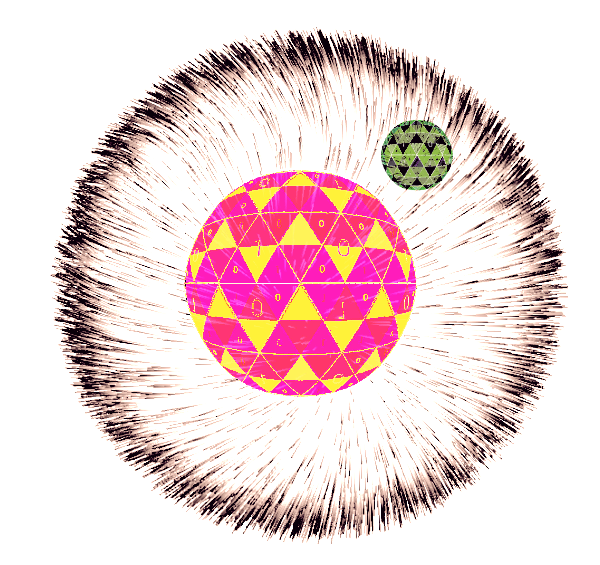
\includegraphics[scale=0.29]{./image/artee-symbiosis.png}
\caption{}
\label{}
\end{figure}


\section{One more thing}
If you are wondering where your old default text is; it has been stored as a template. The template menu can be used to access and restore it. 

\end{document}
\begin{flushleft}\end{flushleft}